\documentclass[12pt, twoside]{article}
\input{../preamble}
\usepackage{pgfplots}
\pgfplotsset{compat=1.18}

\fancyhead[LE]{\thepage}
\fancyhead[RO]{Name: \hspace{4cm} \,\\ \hspace{2.9cm} \,}
\fancyhead[LO]{La Scuola d'Italia / Dr.\ Huson / IB Math \\* 15 April 2026}

\begin{document}
\subsubsection*{6.6 Classwork: The Discriminant and Polynomial Equations (no calculator)}

\begin{enumerate}[itemsep=0.15cm]

%--- Problem 1: Discriminant basics [5 marks] ---
\item[1.] [Maximum mark: 5]

For each quadratic function, find the discriminant $\Delta = b^2 - 4ac$
and state the number of real roots.

\begin{enumerate}[itemsep=0.15cm]
  \item $f(x) = x^2 - 6x + 9$ \hfill [2]
  \item $g(x) = 2x^2 + 3x + 5$ \hfill [2]
  \item State what the discriminant tells you about the graph
  of each function. \hfill [1]
\end{enumerate}

\begin{tikzpicture}
  \draw (0,0) rectangle (15.5,4.5);
  \foreach \y in {1,2,3} \draw[dotted] (0.5,\y)--(15,\y);
\end{tikzpicture}

\vspace{0.3cm}

%--- Problem 2: Discriminant with parameter [6 marks] ---
\item[2.] [Maximum mark: 6]

The equation $x^2 + kx + 9 = 0$ has two equal roots.

\begin{enumerate}[itemsep=0.15cm]
  \item Write down the discriminant in terms of $k$. \hfill [1]
  \item Find the values of $k$. \hfill [2]
  \item For each value of $k$, find the repeated root. \hfill [2]
  \item State the values of $k$ for which the equation has no
  real roots. \hfill [1]
\end{enumerate}

\begin{tikzpicture}
  \draw (0,0) rectangle (15.5,5.5);
  \foreach \y in {1,2,...,4} \draw[dotted] (0.5,\y)--(15,\y);
\end{tikzpicture}

\newpage

%--- Problem 3: Line tangent to parabola [7 marks] ---
\item[3.] [Maximum mark: 7]

The line $y = 2x + c$ is tangent to the parabola $y = x^2 + 1$.

\begin{enumerate}[itemsep=0.15cm]
  \item Show that the $x$-coordinates of any intersection points
  satisfy $x^2 - 2x + (1 - c) = 0$. \hfill [1]
  \item For the line to be tangent, the discriminant must equal zero.
  Find the value of $c$. \hfill [2]
  \item Find the coordinates of the point of tangency. \hfill [2]
  \item On the axes below, sketch the parabola and the tangent line. \hfill [2]
\end{enumerate}

\begin{center}
\begin{tikzpicture}
\begin{axis}[
  axis lines=middle,
  xlabel={$x$},
  ylabel={$y$},
  grid=both,
  grid style={dashed, gray!30},
  xmin=-3, xmax=5,
  ymin=-1, ymax=8,
  xtick={-3,-2,...,5},
  ytick={-1,0,...,8},
  width=10cm,
  height=10cm,
  every axis x label/.style={at={(ticklabel* cs:1.0)}, anchor=west},
  every axis y label/.style={at={(ticklabel* cs:1.0)}, anchor=south},
]
  % Solution curves (commented out)
  %\addplot[thick, domain=-2:4, samples=80] {x^2 + 1};
  %\addplot[thick, dashed, domain=-1:4] {2*x};
  %\node[circle, fill, inner sep=1.8pt] at (axis cs:1,2) {};
\end{axis}
\end{tikzpicture}
\end{center}

\begin{tikzpicture}
  \draw (0,0) rectangle (15.5,6);
  \foreach \y in {1,2,...,5} \draw[dotted] (0.5,\y)--(15,\y);
\end{tikzpicture}

\newpage

%--- Problem 4: Graph interpretation with discriminant [6 marks] ---
\item[4.] [Maximum mark: 6]

The diagram shows the graph of $f(x) = -(x - 3)^2 + 4$.

\begin{center}
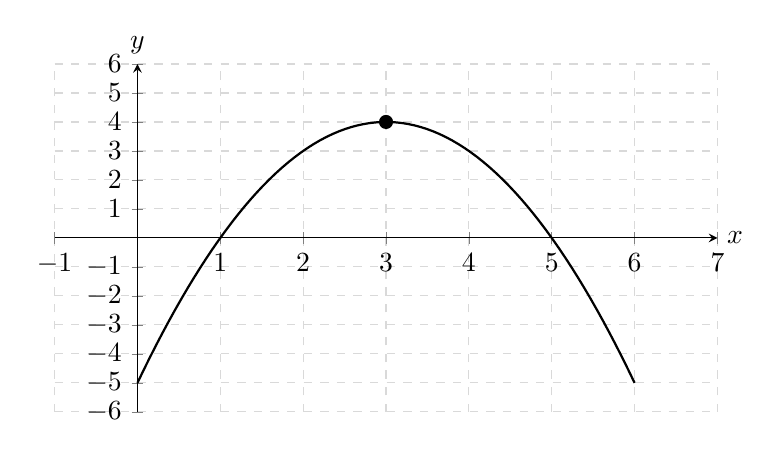
\begin{tikzpicture}
\begin{axis}[
  axis lines=middle,
  xlabel={$x$},
  ylabel={$y$},
  grid=both,
  grid style={dashed, gray!30},
  xmin=-1, xmax=7,
  ymin=-6, ymax=6,
  xtick={-1,0,...,7},
  ytick={-6,-5,...,6},
  width=10cm,
  height=6cm,
  every axis x label/.style={at={(ticklabel* cs:1.0)}, anchor=west},
  every axis y label/.style={at={(ticklabel* cs:1.0)}, anchor=south},
]
  % Parabola: f(x) = -(x-3)^2 + 4 = -x^2 + 6x - 5, vertex (3,4), roots 1 and 5
  \addplot[thick, domain=0:6, samples=80] {-(x-3)^2 + 4};
  % Vertex
  \node[circle, fill, inner sep=1.8pt] at (axis cs:3,4) {};
\end{axis}
\end{tikzpicture}
\end{center}

\begin{enumerate}[itemsep=0.15cm]
  \item Write down the coordinates of the vertex. \hfill [1]
  \item Show that $f(x) = -x^2 + 6x - 5$. \hfill [2]
  \item Find the $x$-intercepts by solving $f(x) = 0$. \hfill [2]
  \item Find the discriminant and explain how it confirms
  your answer to part (c). \hfill [1]
\end{enumerate}

\begin{tikzpicture}
  \draw (0,0) rectangle (15.5,5.5);
  \foreach \y in {1,2,...,4} \draw[dotted] (0.5,\y)--(15,\y);
\end{tikzpicture}

\newpage

%--- Problem 5: Completing the square [6 marks] ---
\item[5.] [Maximum mark: 6]

Consider the function $f(x) = 2x^2 - 8x + 11$.

\begin{enumerate}[itemsep=0.15cm]
  \item Write $f(x)$ in the form $a(x - h)^2 + k$. \hfill [2]
  \item Write down the coordinates of the vertex. \hfill [1]
  \item Use the discriminant to show that $f(x) = 0$ has no
  real solutions. \hfill [2]
  \item Write down the minimum value of $f(x)$. \hfill [1]
\end{enumerate}

\begin{tikzpicture}
  \draw (0,0) rectangle (15.5,5.5);
  \foreach \y in {1,2,...,4} \draw[dotted] (0.5,\y)--(15,\y);
\end{tikzpicture}

\vspace{0.3cm}

%--- Problem 6: Polynomial factoring [6 marks] ---
\item[6.] [Maximum mark: 6]

Let $p(x) = x^3 - 6x^2 + 11x - 6$.

\begin{enumerate}[itemsep=0.15cm]
  \item Show that $(x - 1)$ is a factor of $p(x)$. \hfill [2]
  \item Hence express $p(x)$ as a product of three linear factors. \hfill [2]
  \item Write down all three solutions to $p(x) = 0$. \hfill [1]
  \item Sketch the graph of $y = p(x)$, labelling the
  $x$-intercepts and $y$-intercept. \hfill [1]
\end{enumerate}

\begin{tikzpicture}
  \draw (0,0) rectangle (15.5,6);
  \foreach \y in {1,2,...,5} \draw[dotted] (0.5,\y)--(15,\y);
\end{tikzpicture}

\end{enumerate}
\end{document}
